\documentclass[letterpaper,11pt,twoside,onecolumn,notitlepage]{article}

%% ------------------------------------------------------------------------------------------
%% 1. loading any required packaged here
\usepackage{float,graphicx,grffile}		% graphics
\usepackage{amssymb,amsmath}		% math
\usepackage[margin=0.8in]{geometry}	% document size
\usepackage{natbib}					% bibliography
\usepackage{helvet}					% font
\usepackage{parskip}				% paragraph control
\usepackage{setspace}				% document spacing
\usepackage[unicode=true]{hyperref}	% referencing
\usepackage[T1]{fontenc}
\usepackage{ifxetex,ifluatex}
\usepackage{fixltx2e} 
\usepackage{upquote}
\usepackage{fancyvrb}
\usepackage{listings}
\usepackage{longtable,booktabs}
\usepackage{caption}
\usepackage[section]{placeins}		% figure placement within section only
\usepackage{indentfirst}			% indent first paragraph
\usepackage{nameref,hyperref}		% makes hyper-refs clicky
\usepackage{etoolbox}
\usepackage[left]{lineno}			% line numbers
\usepackage{microtype}				% improves typesetting in LaTeX

%% ------------------------------------------------------------------------------------------
%% 2. defining useful commands
%	- fix paragraph spacing
\raggedbottom

% 	- commands for lists
\providecommand{\tightlist}{%
  \setlength{\itemsep}{0pt}\setlength{\parskip}{0pt}}

% 	- constrain figure size to size of document
\makeatletter
	\def\maxwidth{\ifdim\Gin@nat@width>\linewidth\linewidth\else\Gin@nat@width\fi}
	\def\maxheight{\ifdim\Gin@nat@height>\textheight\textheight\else\Gin@nat@height\fi}
\makeatother
	\setkeys{Gin}{width=0.8\maxwidth,height=0.8\maxheight,keepaspectratio}
\makeatletter
	\def\fps@figure{tbp}
\makeatother

% 	- redefine caption to not include figure numbers (do it manually)
\captionsetup[figure]{labelformat=empty, font=footnotesize}

% 	- turn off numbering of sections
	\setcounter{secnumdepth}{0}

% 	- set paragraph indenting and format
\setlength{\parindent}{0.6cm}
\setlength{\parskip}{3pt plus 2pt minus 1pt}
\setstretch{1.2}

%	- change counting of line numbers
\modulolinenumbers[5]

\bibliographystyle{unsrtnat}

%% ------------------------------------------------------------------------------------------
%% 3. define main text/formating related values
%		- describe the title structure
	\title{Command line tools for a simpler markdown experience}

%		- add authors and affiliations (use numeric referencing regardless of doc class)
\makeatletter
	\let\@fnsymbol\@arabic
\makeatother

	\author{Naveed Ejaz\thanks{Brain and Mind Institiute, University of Western Ontario}}

%% ------------------------------------------------------------------------------------------
%% 4. Main body of document
\begin{document}
	\maketitle


	\hrulefill
	\begin{abstract}
		This document demonstrates a pipeline from going from a markdown
document to nicely formatted pdf or html documents. Typically, a
markdown user would have to understand third party tools like pandoc
which offer ways of converting from markdown to pdf/html. This can be
daunting for novice users, Therefore, I have provided a set of command
line tools that makes the process of providing input to the pandoc
compiler as simple as executing a single line. The command line tools
handle everything from linking the bibliography file to providing
default templates for formatting the desired output files. Templates are
provided for compiling markdown files directly to html using a cascade
style-sheet, and for converting markdown to pdf indirectly by first
compiling to latex and then to pdf. Experience users will be able to
modify the command line tools and the templates that accompany this
tutorial to finely control the output files. Further details are
provided in the make\_pdf and make\_html command line tools. Hopefully,
these command line tools and templates help make the whole markdown
process very simple for you!
	\end{abstract}
	\hrulefill

\linenumbers
	\hypertarget{introduction}{%
\section{Introduction}\label{introduction}}

Markdown offers a way of writing academic papers by separating the
actual text from the formatting of the manuscript. It is fast, and
simple to learn. Since it works on plain text files, it can be used with
github, gitlab or bitbucket for version control. This makes it a very
powerful tool for open-science.

In this tutorial, we will go over a few basics of how to use markdown to
compile plain text into formatted manuscripts that can be shared with
colleagues. This tutorial is not meant to provide a complete overview of
markdown, but rather make it easy for you to go from a plain text
markdown file to a formatted pdf or html output.

\hypertarget{setting-up-pandoc-to-convert-markdown-to-pdfhtml}{%
\subsection{Setting up pandoc to convert markdown to
pdf/html}\label{setting-up-pandoc-to-convert-markdown-to-pdfhtml}}

This tutorial requires that pandoc is correctly installed on the current
machine. The easiest way to get it on a mac is to open a terminal
window, and use the brew project dependency manager to install the
pandoc. To do this, open up a terminal window, and type the following
commands:
\texttt{brew\ install\ pandoc\ pandoc-citeproc\ pandoc-crossref}.

\hypertarget{quick-introduction-to-markdown}{%
\subsection{Quick introduction to
markdown}\label{quick-introduction-to-markdown}}

Once you have pandoc all setup, lets take a look at what options
markdown has to offer:

We can make either number lists,

\begin{enumerate}
\def\labelenumi{\arabic{enumi}.}
\tightlist
\item
  Superscripts and subscripts can be inserted as x\textsuperscript{i} or
  x\textsubscript{i}\\
\item
  Equations can be inserted in-line using \(y_x\), or alternatively they
  can be inserted as an array:
\end{enumerate}

\[ y = t_i + x_i  \]

\hypertarget{citations-with-markdown}{%
\subsection{Citations with markdown}\label{citations-with-markdown}}

Markdown and pandoc offers a quick and easy way to add citations to your
manuscript. All you need is a bibliography in bibtex format, and then
the citation can be added to the document using the
\texttt{{[}@cite\_key{]}} notation. For example, a citation can be
inserted in full like this (Ejaz et al. 2017), or alternatively the
author can be suppressed like by using the minus notation
\texttt{{[}-@cite\_key{]}} like this (2017).

\hypertarget{images-and-hyper-links}{%
\subsection{Images and hyper-links}\label{images-and-hyper-links}}

Markdown also offers an easy way to insert hyper-links into your
document (example: \href{http://www.google.com}{Google}), as well as
inserting images with typeset captions.

\begin{figure}
\centering
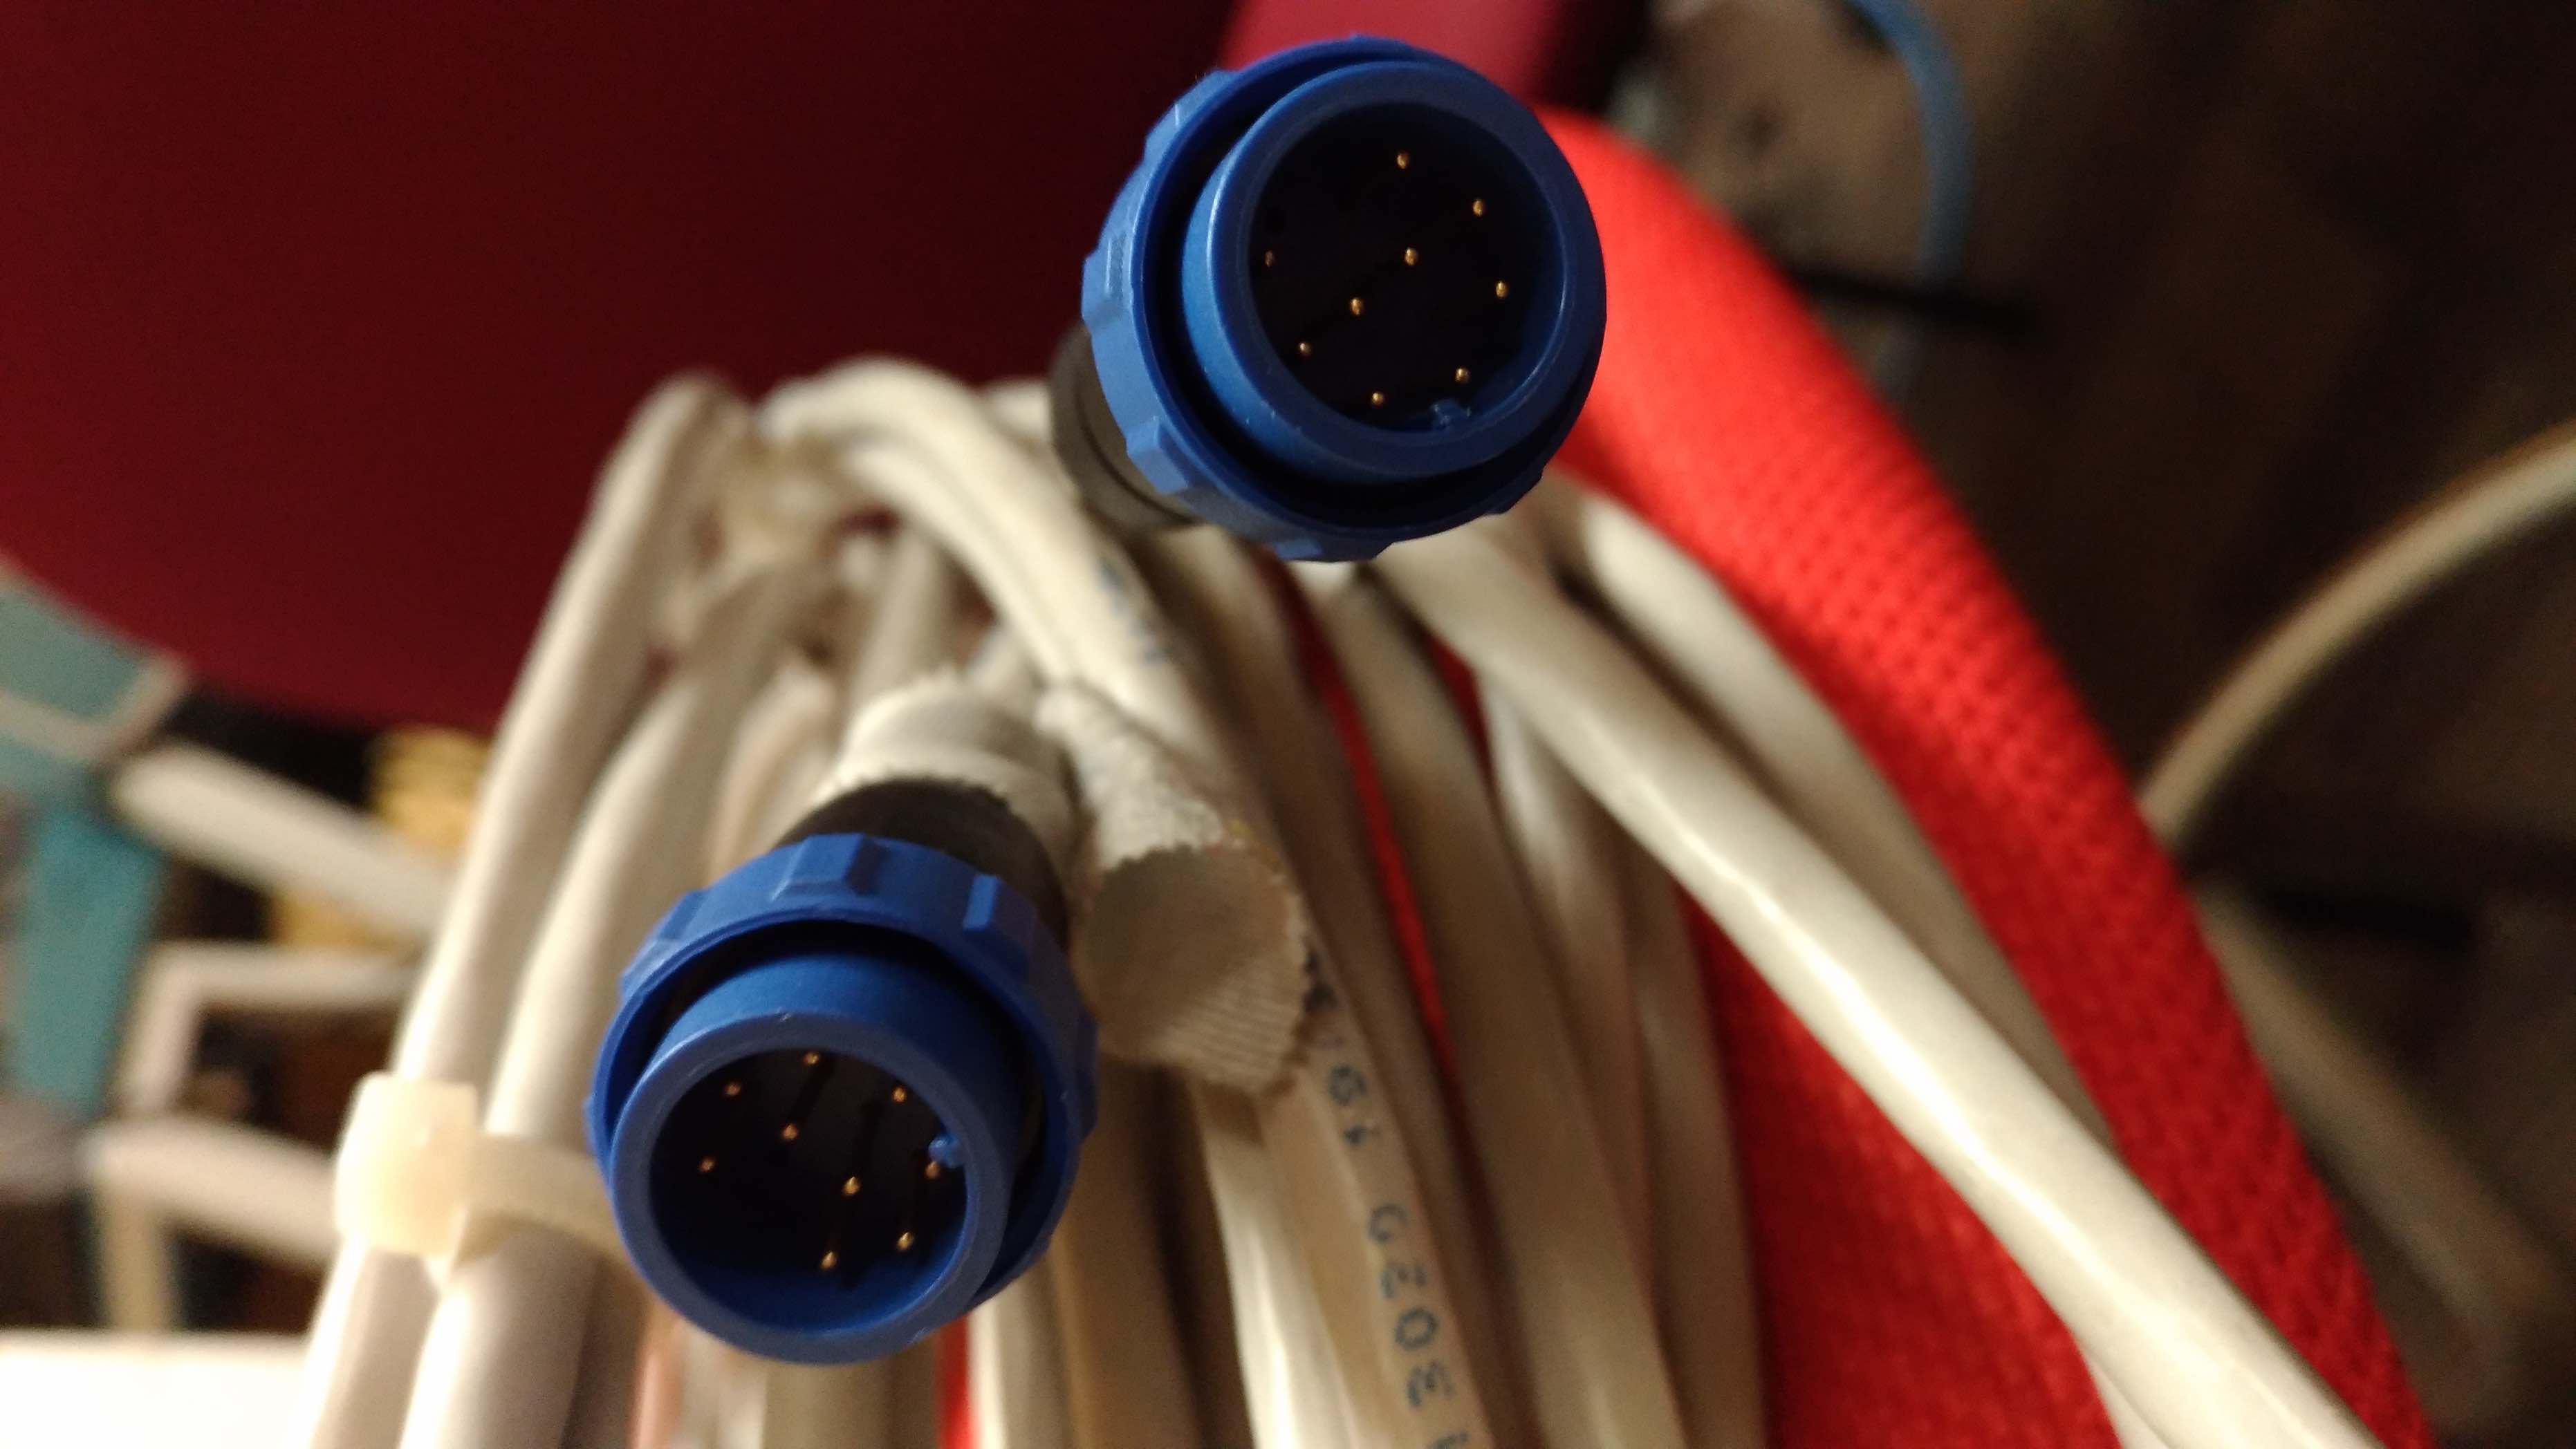
\includegraphics{img.jpg}
\caption{Figures and captions are nicely typeset in markdown}
\end{figure}

\hypertarget{generating-pdf-and-html-files}{%
\subsection{Generating pdf and html
files}\label{generating-pdf-and-html-files}}

To make going from markdowns plan files to nicely formatted pdf and html
requires understanding the details of how pandoc works. For most, this
can be a big hassle. Therefore, I have provided you with two scripts
alongside this template which makes the whole process as simple as
running one command. To generate pdf files, open a terminal window, and
navigate to the directory with this file, and execute the command
\texttt{./make\_pdf} to generate pdf files and \texttt{./make\_html} to
generate html files, respectively.

\hypertarget{references}{%
\section*{References}\label{references}}
\addcontentsline{toc}{section}{References}

\hypertarget{refs}{}
\leavevmode\hypertarget{ref-Diedrichsen:2017fy}{}%
\textbf{Diedrichsen J}, \textbf{Yokoi A}, \textbf{Arbuckle S}. Pattern
Component Modeling: A Flexible Approach For Understanding The
Representational Structure Of Brain Activity Patterns. \emph{bioRxiv}..

\leavevmode\hypertarget{ref-Ejaz:2017fo}{}%
\textbf{Ejaz N}, \textbf{Xu J}, \textbf{Branscheidt M}, \textbf{Hertler
B}, \textbf{Schambra H}, \textbf{Widmer M}, \textbf{Faria AV},
\textbf{Harran M}, \textbf{Cortes JC}, \textbf{Kim N}, \textbf{Kitago
T}, \textbf{Celnik PA}, \textbf{Luft A}, \textbf{Krakauer JW},
\textbf{Diedrichsen J}. Finger recruitment patterns during mirror
movements suggest two systems for hand recovery after stroke.
\emph{bioRxiv}..

\end{document}